\section{前沿的计算}
\label{sec:moo-front-computation}

决策者常常要先看到各种取舍，再做决定。这就要求算出一组候选，而不是一个点。单次标量化或一次多梯度下降都只给出前沿上的一点，所以要么反复求解，要么同时维护多个候选。本节分别讨论这两条路：由偏好参数驱动的重复求解，和由支配关系驱动的群体搜索。

\subsection{参数扫描}
\label{sec:moo-scan}

把权重、阈值或参考点变化一遍，每次解一个单目标问题，能否得到一组分布合理的候选？这一小节要说明，参数均匀并不等于前沿均匀，并给出按空缺补充求解的办法。

\paragraph{均匀的参数不等于均匀的前沿}
在例~\eqref{eq:moo-iso}上，由式~\eqref{eq:moo-iso-weighted}，取$w=0,1/4,1/2,3/4,1$，得到前沿上的五个点
\[
 (1,0),\quad(0.5625,0.0625),\quad(0.25,0.25),\quad(0.0625,0.5625),\quad(0,1).
\]
相邻两点的距离依次约为$0.442,0.364,0.364,0.442$，不算均匀，但差得不多。

如果两个目标的尺度悬殊，差别就大了。例~\eqref{eq:moo-mgda-example}的加权和有显式解，由$w\bm{g}_1+(1-w)\bm{g}_2=\bm{0}$逐分量解出
\begin{equation}
 \bm{x}(w)=\Bigl(4(1-w),\ \frac{3(1-w)}{8w+1}\Bigr).
 \label{eq:moo-mgda-weighted}
\end{equation}
图~\ref{fig:moo-scan-gaps}(a)是$11$个均匀的$w$所对应的点，点都挤在左上方，右下方有一个大空缺。按目标范围归一化后，相邻点间距最大约为$0.665$，最小约为$0.089$。

\begin{BookInlineFigure}
  \centering
  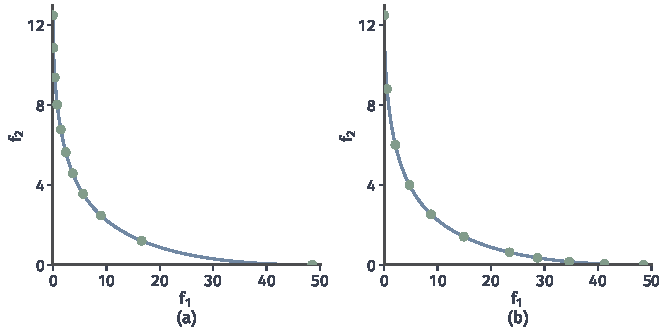
\includegraphics[width=112mm]{figures/05-optimization/07-multiple-criteria-and-nested-optimization/matplotlib/moo-scan-gaps/figure.pdf}
  \caption{例~\eqref{eq:moo-mgda-example}前沿上的$11$个候选。(a)$w$在$[0,1]$上均匀取值，点集中在左上方。(b)按最大空缺逐次补点，权重取空缺两端连线的法向。两图的端点相同。}
  \label{fig:moo-scan-gaps}
\end{BookInlineFigure}

\paragraph{按空缺补点}
既然均匀的参数靠不住，就让已经算出的点来决定下一个参数。对凸前沿，下面的过程很自然。

先用两个端点权重算出两端的点。然后反复做这样一步：找出归一化后间距最大的相邻两点$\bm{p},\bm{q}$，取这两点连线的法向作为新的权重，
\begin{equation}
 w=\frac{\lvert q_2-p_2\rvert}{\lvert q_2-p_2\rvert+\lvert q_1-p_1\rvert},
 \label{eq:moo-chord-weight}
\end{equation}
求解相应的加权和，把新点插进去。新权重下，支撑线与连线平行，解是这段前沿上离连线最远的点。若解不比$\bm{p},\bm{q}$的连线更靠左下，说明这一段已经没有新的支撑点，把这段标记为完成。

在例~\eqref{eq:moo-iso}上走几步。两端是$(0,1)$和$(1,0)$，由式~\eqref{eq:moo-chord-weight}得$w=1/2$，由式~\eqref{eq:moo-iso-weighted}得新点$(1/4,1/4)$。

在$(0,1)$与$(1/4,1/4)$之间，两个差值是$3/4$和$1/4$，权重为
\[
 w=\frac{3/4}{3/4+1/4}=\frac34,
\]
新点是$(1/16,9/16)$。在$(1/4,1/4)$与$(1,0)$之间，同理$w=1/4$，新点是$(9/16,1/16)$。五个点到此与均匀权重的结果相同，继续补点时，算法开始根据实际空缺分配求解次数。

在例~\eqref{eq:moo-mgda-example}上，按这种做法得到图~\ref{fig:moo-scan-gaps}(b)，归一化间距的最大值降到约$0.296$，最小值约为$0.111$，同样$11$次求解分布均匀得多。这里的选取规则只用到已算出的点，但法向的含义依赖目标尺度，所以要先说明归一化的参考范围。

\paragraph{用邻近问题的解作初值}
相邻参数的解通常相隔不远，这启发了用上一个解作下一个问题的初值，称为\term{热启动}（warm start）。图~\ref{fig:moo-warm-start}比较了两种做法：用梯度法解$39$个加权子问题，步长取该子问题的$1/L$，梯度范数降到$10^{-3}$为止。

\begin{BookInlineFigure}
  \centering
  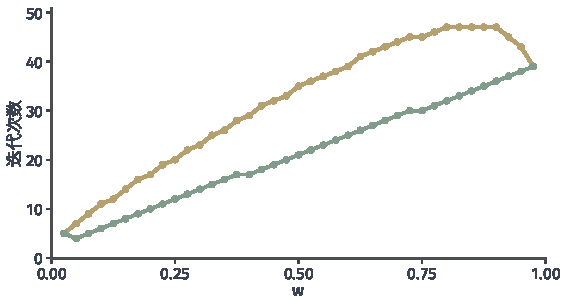
\includegraphics[width=96mm]{figures/05-optimization/07-multiple-criteria-and-nested-optimization/matplotlib/moo-warm-start/figure.pdf}
  \caption{例~\eqref{eq:moo-mgda-example}的$39$个加权子问题所用的梯度法迭代次数，$w$每步增加$0.025$。黄线是每次从$(0,2)$冷启动，共$1232$步；绿线是从上一个解热启动，共$826$步。}
  \label{fig:moo-warm-start}
\end{BookInlineFigure}

总迭代次数从$1232$降到$826$。线性收敛的方法从更好的初值出发，节省的是迭代次数对数中的一项，收敛速率本身不变，所以这里只节省三分之一左右，高精度要求下比例还会更小。

\paragraph{保存非支配候选}
扫描得到的点不一定都有用：求解可能不精确，并列解可能只是弱Pareto最优点。所以要维护一个\term{非支配存档}（non-dominated archive）。新点进来时，若被存档中的点支配就丢弃；否则把它支配的旧点删掉，再加入存档。

按$A,E,B,F,C,D$的顺序把式~\eqref{eq:moo-candidates}中的候选送入存档。$A$进入；$E$与$A$不可比，进入；$B$支配$E$，把$E$换成$B$；$F$与已有的点不可比，进入；$C$也进入；$D$支配$F$，把$F$换成$D$。最后得到$\{A,B,C,D\}$。

\paragraph{可达性的限制仍然存在}
无论参数取得多细，每种标量化能到达的点不会变多。图~\ref{fig:moo-scan-compare}在带凹陷的前沿上各取九个均匀的参数。加权和在$w\geq0.7$的三次求解全落到端点，凹陷段里一个点也没有，点从$(0.577,0.183)$直接跳到$(0.206,0.633)$。阈值约束和加权Chebyshev都把点放进了凹陷。

\begin{BookInlineFigure}
  \centering
  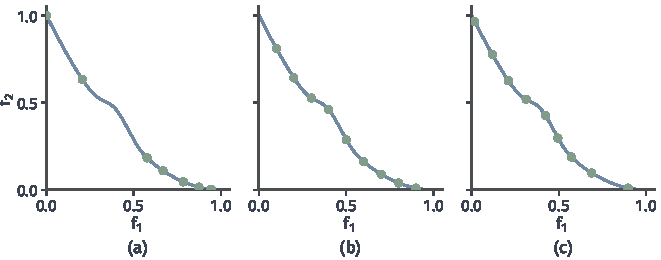
\includegraphics[width=112mm]{figures/05-optimization/07-multiple-criteria-and-nested-optimization/matplotlib/moo-scan-compare/figure.pdf}
  \caption{带凹陷的前沿上三种标量化的扫描，每种取九个均匀参数。(a)加权和，$w=0.1,\ldots,0.9$，$w\geq0.7$的三点重合在左端。(b)阈值约束，$\tau=0.1,\ldots,0.9$。(c)加权Chebyshev，$\bm{z}=(-0.1,-0.1)$，$\bm{w}=(w,1-w)$。}
  \label{fig:moo-scan-compare}
\end{BookInlineFigure}

所以，在非凸前沿上，要用阈值约束或加权Chebyshev来做扫描，并且每次求解都要检查是否达到全局最优。若子问题只解到局部最优，定理~\ref{thm:moo-threshold}和定理~\ref{thm:moo-chebyshev}的保证都不再适用。

\subsection{非支配排序}
\label{sec:moo-nsga}

参数扫描每次只优化一个点。能不能让一批候选同时朝前沿移动，并在前沿上散开？这一小节以NSGA-II为例，说明怎样把第~\ref{chap:random-search}章的种群搜索改造成服务前沿近似的算法。

\paragraph{主要思想}
\term{NSGA-II}（non-dominated sorting genetic algorithm II）沿用遗传算法的框架，维护一个规模为$N$的种群，变异和重组都与第~\ref{chap:random-search}章相同。要改造的是选择：单目标时按代价排序就能分出好坏，这里目标是向量，排序要回答两个问题。

第一个问题是谁离前沿更近。把种群按支配关系分层，不被任何个体支配的点是第一层；把第一层去掉后，剩下的点中不被支配的是第二层，依此类推。这个过程称为\term{非支配排序}（non-dominated sorting）。层号越小越靠近前沿。

第二个问题是同一层内谁应当保留。同一层的点互不支配，排不出优劣，但我们希望点在前沿上散开。所以优先保留周围比较空的点，用\term{拥挤距离}（crowding distance）度量。

对一层的点集，按目标$k$排序，设点$\bm{y}$的前后邻点为$\bm{y}^-$和$\bm{y}^+$，该层在目标$k$上的范围为$R_k$，拥挤距离是
\begin{equation}
 D(\bm{y})=\sum_{k=1}^m\frac{y_k^+-y_k^-}{R_k}.
 \label{eq:moo-crowding}
\end{equation}
每个目标上的两个端点取$D=\infty$，这样最大的和最小的值总被保留。式~\eqref{eq:moo-crowding}是以邻点为角的长方体的周长的一种度量。除以$R_k$使不同尺度的目标能够相加，也因此依赖该层的取值范围。

还有一个改造：下一代从亲代与后代的并集中选出，这就是\term{精英保留}（elitism）的做法，和第~\ref{chap:random-search}章的$(\mu+\lambda)$选择相同。好的亲代不会因后代变差而丢失。图~\ref{fig:moo-nsga-flow}是一代的流程。

\begin{BookInlineFigure}
  \centering
  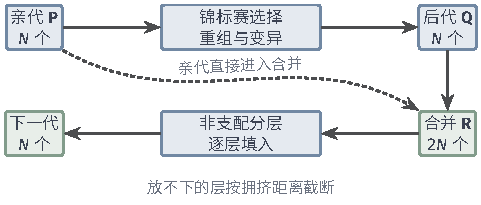
\includegraphics[width=81.5mm]{figures/05-optimization/07-multiple-criteria-and-nested-optimization/tikz/moo-nsga-flow/figure.pdf}
  \caption{NSGA-II的一代。亲代经锦标赛选择、重组与变异产生后代，亲代与后代合并成$2N$个候选，分层后逐层填入下一代，最后放不下的那一层按拥挤距离从大到小取。}
  \label{fig:moo-nsga-flow}
\end{BookInlineFigure}

\needspace{6\baselineskip}
\paragraph{变量}
\begin{itemize}
 \item 种群$\bm{P}$，$N$个候选及其目标向量，每个候选的层号与拥挤距离；
 \item 后代$\bm{Q}$，$N$个候选；合并的集合$\bm{R}=\bm{P}\cup\bm{Q}$；
 \item 分层计算中的辅助量：$S_{\bm{p}}$是$\bm{p}$支配的点集，$n_{\bm{p}}$是支配$\bm{p}$的点数。
\end{itemize}

\paragraph{初始化}
随机产生$N$个候选并评价，分层并计算拥挤距离。下面用例子说明一代中的选择。假设合并后得到八个候选，它们是式~\eqref{eq:moo-candidates}的六个点，加上
\[
 G=(3,7),\qquad H=(6,7).
\]

\needspace{6\baselineskip}
\paragraph{每轮更新}
\begin{enumerate}
 \item 产生后代：用二元锦标赛选亲代，比较时层号小者胜，层号相同时拥挤距离大者胜；再做重组和变异。例中假定后代已经产生并合并。

 \item 合并亲代和后代，对每一点计算$n_{\bm{p}}$和$S_{\bm{p}}$。例中
 \[
  n_A=n_B=n_C=n_D=0,\quad n_E=2,\quad n_F=n_G=1,\quad n_H=5.
 \]
 $E$被$B,C$支配，$F$被$D$支配，$G$被$B$支配，$H$被$B,C,D,E,G$支配。

 \item 分层：$n_{\bm{p}}=0$的点组成第一层，把它们支配的点的$n$减一，$n$减到零的点组成下一层，依此类推。例中第一层是$\{A,B,C,D\}$。把它们去掉后$n_E=n_G=n_F=0$，第二层是$\{E,F,G\}$，第三层是$\{H\}$，见图~\ref{fig:moo-nsga-layers}(a)。

 \item 逐层填入下一代，直到某一层放不下。例中取$N=6$，第一层四个点全部进入，还差两个名额。

 \item 放不下的那一层，计算拥挤距离~\eqref{eq:moo-crowding}，按从大到小取够。例中第二层$G,E,F$按$f_1$排序是$G,E,F$，$G,F$是端点，距离为无穷；$E$的距离是
 \[
  D(E)=\frac{7-3}{7-3}+\frac{7-1}{7-1}=2.
 \]
 所以取$G$和$F$，$E$被淘汰。下一代是$\{A,B,C,D,F,G\}$。
\end{enumerate}

这一例也提醒我们，$F$虽然只是弱Pareto最优点，却因为端点的身份进入了下一代。分层只反映种群内部的关系。

截断也可能发生在第一层。若$N=3$，第一层四个点要留三个。$A$和$D$是端点，距离为无穷。其余两点的距离由式~\eqref{eq:moo-crowding}算出：
\[
 D(B)=\frac{4-1}{5}+\frac{8-4}{7}\approx1.171,\qquad
 D(C)=\frac{6-2}{5}+\frac{5-1}{7}\approx1.371.
\]
所以保留$A,C,D$，淘汰$B$，图~\ref{fig:moo-nsga-layers}(b)画出了这两个长方形。$C$在加权和下永远选不上，在这里却因为不拥挤而被留下：种群搜索的比较只用支配和距离，不要求支撑。

\begin{BookInlineFigure}
  \centering
  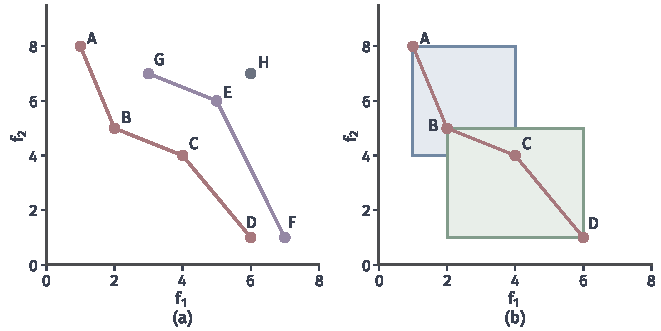
\includegraphics[width=112mm]{figures/05-optimization/07-multiple-criteria-and-nested-optimization/matplotlib/moo-nsga-layers/figure.pdf}
  \caption{八个候选的非支配排序与拥挤距离。(a)红色、紫色、灰色依次是第一、二、三层。(b)第一层内$B$与$C$的拥挤长方形，分别以$A,C$和$B,D$为角，$C$的长方形更大。}
  \label{fig:moo-nsga-layers}
\end{BookInlineFigure}

\paragraph{运行效果}
一代中比较支配关系的开销是$O(mN^2)$，拥挤距离的排序是$O(mN\log N)$，加上$N$次目标评价。目标评价昂贵时，主要开销是评价的次数。

图~\ref{fig:moo-nsga-run}是在一个五维问题上的实际运行。取$\bm{x}\in[0,1]^5$，
\begin{equation}
 f_1=x_1,\quad \gamma=1+\frac{9}{4}\sum_{j=2}^{5}x_j,\quad f_2=\gamma\Bigl(1-\bigl(f_1/\gamma\bigr)^2\Bigr).
 \label{eq:moo-zdt}
\end{equation}
当$x_2=\cdots=x_5=0$时$\gamma=1$，$f_2=1-f_1^2$，这就是式~\eqref{eq:moo-concave}的抛物线前沿。其余变量把点往上推。种群规模为$40$，运行$200$代，随机种子固定。

\begin{BookInlineFigure}
  \centering
  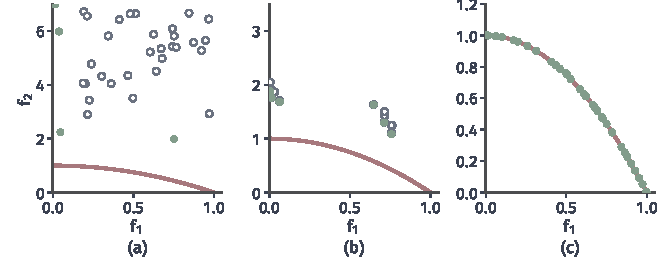
\includegraphics[width=112mm]{figures/05-optimization/07-multiple-criteria-and-nested-optimization/matplotlib/moo-nsga-run/figure.pdf}
  \caption{NSGA-II在式~\eqref{eq:moo-zdt}上的种群，种群规模$40$。红线是真实前沿，绿点是当前种群的第一层，空心点是其余个体。(a)初始种群。(b)第$10$代，第一层有$12$个点，互不支配，但离前沿还很远。(c)第$200$代，$40$个点都在前沿附近。三幅图的纵轴范围不同。}
  \label{fig:moo-nsga-run}
\end{BookInlineFigure}

第$10$代的$12$个点互不支配，却离真实前沿还很远。这正是必须记住的一点：有限种群内部互不支配，不能说明它们是Pareto最优的。算法没有全局保证，它的结果要靠第~\ref{sec:moo-front-evaluation}节的量来检查。加权和扫描在这个问题上只能得到两个端点，这里的种群搜索能把点散布到整条前沿上，这是它的优势。
